\RequirePackage{amsmath}
\documentclass[runningheads]{llncs}
%
\usepackage[T1]{fontenc}
\usepackage{float}
\usepackage{graphicx}
\usepackage{subcaption}
\usepackage[inline]{enumitem}
% Used for displaying a sample figure. If possible, figure files should
% be included in EPS format.
%
% If you use the hyperref package, please uncomment the following two lines
% to display URLs in blue roman font according to Springer's eBook style:
%\usepackage{color}
%\renewcommand\UrlFont{\color{blue}\rmfamily}
%\urlstyle{rm}

\usepackage{tikz} 
\usetikzlibrary{
    calc,
    decorations.pathmorphing,
    decorations.pathreplacing, 
    shapes.geometric, 
} 

\usepackage{macros}
\usepackage[capitalise,noabbrev]{cleveref}

\begin{document}
%
\title{Realizing Graphs with Cut Constraints}
% Tikz
%\titlerunning{Abbreviated paper title}
% If the paper title is too long for the running head, you can set
% an abbreviated paper title here
%

\author{
Vítor Gomes Chagas\inst{1}\orcidID{0000-0002-6506-4174}
\and \\
Samuel Plaça de Paula\inst{1}\orcidID{0009-0005-5970-2984}
\and \\
Greis Yvet Oropeza Quesquén\inst{1}\orcidID{0000-0003-0112-8009}
\and \\
Lucas de Oliveira Silva\inst{1}\orcidID{0000-0002-7846-5903}
\and \\
Uéverton dos Santos Souza\inst{2,3}\orcidID{0000-0002-5320-9209}
}

\authorrunning{V. G. Chagas et al.}
% First names are abbreviated in the running head.
% If there are more than two authors, 'et al.' is used.
%

\institute{
Instituto de Computação, Universidade Estadual de Campinas, Campinas, Brazil\\
\email{vitor.chagas@ic.unicamp.br} \\
\email{s233554@dac.unicamp.br} \\
\email{greis.quesquen@ic.unicamp.br} \\
\email{lucas.oliveira.silva@ic.unicamp.br} \\
\and
IMPA, Instituto de Matemática Pura e Aplicada, Rio de Janeiro, Brazil\\
\and
Instituto de Computação, Universidade Federal Fluminense, Niterói, Brazil\\
\email{ueverton.souza@impatech.org.br}}

%
\maketitle % typeset the header of the contribution
%
\begin{abstract}
%The abstract should briefly summarize the contents of the paper in 150--250 words.

Given a finite non-decreasing sequence $\texttt{d}=(d_1,\ldots,d_n)$ of natural numbers, % such that $d_1\geq d_2 \geq \ldots \geq d_n$, 
the \GRfull~problem asks whether \texttt{d} is a graphic sequence, i.e., there exists a labeled simple graph such that $(d_1,\ldots,d_n)$ is the degree sequence of this graph. Such a problem can be solved in polynomial time due to the Erd\H{o}s and Gallai characterization of graphic sequences. 
%In particular, \texttt{d} is graphic if and only if $\sum\limits_{i=1}^n d_i$ is even and $\sum\limits_{i=1}^k d_k \leq k(k-1) + \sum\limits_{j=k+1}^n\min\{k,d_j\}$ for all $k\in\{1,\ldots,n\}$.
Since vertex degree is the size of a trivial edge cut, we consider a natural generalization of \GRfull, where we are given a finite sequence $\texttt{d}=(d_1,\ldots,d_n)$ of natural numbers (representing the trivial edge cut sizes) and a list of nontrivial cut constraints $\call$ composed of pairs $(S_j,\ell_j)$ where $S_j\subset \{v_1,\ldots,v_n\}$, and $\ell_j$ is a natural number.
%
In such a problem, we are asked whether there is a simple graph with vertex set $V=\{v_1,\ldots,v_n\}$ such that $v_i$ has degree $d_i$ and $\partial(S_j)$ is an edge cut of size $\ell_j$, for each $(S_j,\ell_j)\in \call$. We show that such a problem is polynomial-time solvable whenever each $S_j$ has size at most three. Conversely, assuming P~$\neq$~NP, we prove that it cannot be solved in polynomial time when $\call$ contains pairs with sets of size four, and our hardness result holds even assuming that each $d_i$ of \texttt{d} equals $1$. 

\keywords{Graph realization \and Degree sequence \and Graph factor}
\end{abstract}
%
%
%
% guidelines do CIAC deteminam que a página de título contenha só até o abstract
\newpage

\section{Introduction}

Despite the remarkable capabilities of large language models (LLMs)~\cite{DBLP:conf/emnlp/QinZ0CYY23,DBLP:journals/corr/abs-2307-09288}, they often inevitably exhibit hallucinations due to incorrect or outdated knowledge embedded in their parameters~\cite{DBLP:journals/corr/abs-2309-01219, DBLP:journals/corr/abs-2302-12813, DBLP:journals/csur/JiLFYSXIBMF23}.
Given the significant time and expense required to retrain LLMs, there has been growing interest in \emph{model editing} (a.k.a., \emph{knowledge editing})~\cite{DBLP:conf/iclr/SinitsinPPPB20, DBLP:journals/corr/abs-2012-00363, DBLP:conf/acl/DaiDHSCW22, DBLP:conf/icml/MitchellLBMF22, DBLP:conf/nips/MengBAB22, DBLP:conf/iclr/MengSABB23, DBLP:conf/emnlp/YaoWT0LDC023, DBLP:conf/emnlp/ZhongWMPC23, DBLP:conf/icml/MaL0G24, DBLP:journals/corr/abs-2401-04700}, 
which aims to update the knowledge of LLMs cost-effectively.
Some existing methods of model editing achieve this by modifying model parameters, which can be generally divided into two categories~\cite{DBLP:journals/corr/abs-2308-07269, DBLP:conf/emnlp/YaoWT0LDC023}.
Specifically, one type is based on \emph{Meta-Learning}~\cite{DBLP:conf/emnlp/CaoAT21, DBLP:conf/acl/DaiDHSCW22}, while the other is based on \emph{Locate-then-Edit}~\cite{DBLP:conf/acl/DaiDHSCW22, DBLP:conf/nips/MengBAB22, DBLP:conf/iclr/MengSABB23}. This paper primarily focuses on the latter.

\begin{figure}[t]
  \centering
  \includegraphics[width=0.48\textwidth]{figures/demonstration.pdf}
  \vspace{-4mm}
  \caption{(a) Comparison of regular model editing and EAC. EAC compresses the editing information into the dimensions where the editing anchors are located. Here, we utilize the gradients generated during training and the magnitude of the updated knowledge vector to identify anchors. (b) Comparison of general downstream task performance before editing, after regular editing, and after constrained editing by EAC.}
  \vspace{-3mm}
  \label{demo}
\end{figure}

\emph{Sequential} model editing~\cite{DBLP:conf/emnlp/YaoWT0LDC023} can expedite the continual learning of LLMs where a series of consecutive edits are conducted.
This is very important in real-world scenarios because new knowledge continually appears, requiring the model to retain previous knowledge while conducting new edits. 
Some studies have experimentally revealed that in sequential editing, existing methods lead to a decrease in the general abilities of the model across downstream tasks~\cite{DBLP:journals/corr/abs-2401-04700, DBLP:conf/acl/GuptaRA24, DBLP:conf/acl/Yang0MLYC24, DBLP:conf/acl/HuC00024}. 
Besides, \citet{ma2024perturbation} have performed a theoretical analysis to elucidate the bottleneck of the general abilities during sequential editing.
However, previous work has not introduced an effective method that maintains editing performance while preserving general abilities in sequential editing.
This impacts model scalability and presents major challenges for continuous learning in LLMs.

In this paper, a statistical analysis is first conducted to help understand how the model is affected during sequential editing using two popular editing methods, including ROME~\cite{DBLP:conf/nips/MengBAB22} and MEMIT~\cite{DBLP:conf/iclr/MengSABB23}.
Matrix norms, particularly the L1 norm, have been shown to be effective indicators of matrix properties such as sparsity, stability, and conditioning, as evidenced by several theoretical works~\cite{kahan2013tutorial}. In our analysis of matrix norms, we observe significant deviations in the parameter matrix after sequential editing.
Besides, the semantic differences between the facts before and after editing are also visualized, and we find that the differences become larger as the deviation of the parameter matrix after editing increases.
Therefore, we assume that each edit during sequential editing not only updates the editing fact as expected but also unintentionally introduces non-trivial noise that can cause the edited model to deviate from its original semantics space.
Furthermore, the accumulation of non-trivial noise can amplify the negative impact on the general abilities of LLMs.

Inspired by these findings, a framework termed \textbf{E}diting \textbf{A}nchor \textbf{C}ompression (EAC) is proposed to constrain the deviation of the parameter matrix during sequential editing by reducing the norm of the update matrix at each step. 
As shown in Figure~\ref{demo}, EAC first selects a subset of dimension with a high product of gradient and magnitude values, namely editing anchors, that are considered crucial for encoding the new relation through a weighted gradient saliency map.
Retraining is then performed on the dimensions where these important editing anchors are located, effectively compressing the editing information.
By compressing information only in certain dimensions and leaving other dimensions unmodified, the deviation of the parameter matrix after editing is constrained. 
To further regulate changes in the L1 norm of the edited matrix to constrain the deviation, we incorporate a scored elastic net ~\cite{zou2005regularization} into the retraining process, optimizing the previously selected editing anchors.

To validate the effectiveness of the proposed EAC, experiments of applying EAC to \textbf{two popular editing methods} including ROME and MEMIT are conducted.
In addition, \textbf{three LLMs of varying sizes} including GPT2-XL~\cite{radford2019language}, LLaMA-3 (8B)~\cite{llama3} and LLaMA-2 (13B)~\cite{DBLP:journals/corr/abs-2307-09288} and \textbf{four representative tasks} including 
natural language inference~\cite{DBLP:conf/mlcw/DaganGM05}, 
summarization~\cite{gliwa-etal-2019-samsum},
open-domain question-answering~\cite{DBLP:journals/tacl/KwiatkowskiPRCP19},  
and sentiment analysis~\cite{DBLP:conf/emnlp/SocherPWCMNP13} are selected to extensively demonstrate the impact of model editing on the general abilities of LLMs. 
Experimental results demonstrate that in sequential editing, EAC can effectively preserve over 70\% of the general abilities of the model across downstream tasks and better retain the edited knowledge.

In summary, our contributions to this paper are three-fold:
(1) This paper statistically elucidates how deviations in the parameter matrix after editing are responsible for the decreased general abilities of the model across downstream tasks after sequential editing.
(2) A framework termed EAC is proposed, which ultimately aims to constrain the deviation of the parameter matrix after editing by compressing the editing information into editing anchors. 
(3) It is discovered that on models like GPT2-XL and LLaMA-3 (8B), EAC significantly preserves over 70\% of the general abilities across downstream tasks and retains the edited knowledge better.
% \newpage

\section{Preliminaries}
\label{sec:preliminaries}

Let $S$ be a set of vertices of a graph $G=(V, E)$.
We denote the total degree of vertices in $S$ by $d(S) = \sum_{u \in S} d_u$, where $d_u$ represents the degree of vertex $u$.
A simple observation is that the size of the edge cut $\partial(S)$ is determined by the degree of the vertices in $S$ and the edges between vertices of $S$.
If there are $k$ edges between vertices of $S$, then $\size{\partial(S)}=d(S)- 2k$.
%
Since the number of edges in $S$ may vary from $0$ to $\binom{\size{S}}{2}$, a necessary condition for the realizability of an \GRC{} instance is as follows.

\begin{remark}
\label{thm:feasible_cut_sizes}
    A \GRC{} instance $(\texttt{d}, \call)$ is realizable only if, for each cut $(S, \ell) \in \call$, we have $\ell \in \set{ d(S) - 2k : 0 \leq k \leq \binom{\size{S}}{2} }$.
\end{remark}

Since this condition is easily verifiable, we assume henceforth that it holds for any \GRC{} instance. In particular, for cuts of size two, this observation implies that only two feasible values are possible, determining whether an edge must exist between the corresponding vertices, as detailed below.

\begin{remark}
\label{thm:fixed_forbidden_edges}
    Given an instance $I = (\texttt{d}, \call)$ of \GRC{}, in any realization $G$ of $I$, if $(\set{u, v}, d_u + d_v - 2) \in \call$, then $uv \in E(G)$, and if $(\set{u, v}, d_u + d_v) \in \call$, then $uv \notin E(G)$.
\end{remark}

Based on this, we say that an edge $uv$ is \textit{fixed} if $(\set{u, v}, d_u + d_v - 2) \in \call$ and is \textit{forbidden} if $(\set{u, v}, d_u + d_v) \in \call$.
We apply similar terminology when constructing an instance of \GRC{}.
Given an instance $(\texttt{d}, \call)$ of \GRC{}, to \textit{fix} or \textit{forbid} an edge $uv$ means adding the cut $(\set{u, v}, d_u + d_v - 2)$ or $(\set{u, v}, d_u + d_v)$ to $\call$, respectively.

\cref{thm:fixed_forbidden_edges} implies that the \GRC{} problem, when limited to cuts of size two, is equivalent to the \GR{} problem with added constraints: a subset of edges is fixed, and another disjoint one is forbidden. Moreover, we can simplify the problem by focusing only on forbidden edges by reducing the degree of vertices incident to fixed edges and then marking those edges as forbidden.
%
Formally, given an instance $(\texttt{d}, \call)$ and a cut $(\set{u, v}, d_u + d_v - 2) \in \call$, in which case the edge $uv$ is fixed, we can produce an equivalent instance $(\texttt{d}', \call')$ as follows.  For all $i \notin \{u, v\}$  set $d'_i = d_i$. Reduce $d'_u = d_u - 1$ and   $d'_v = d_v - 1$;  
%\begin{align*}
    % \begin{cases}
    %     d'_i = d_i, &\text{ if  $i \notin \{u, v\}$ }\\
    %     d'_u = d_u - 1 \\
    %     d'_v = d_v - 1 
    % \end{cases}
    %
    % d'_i &= d_i, &\mbox{ if  }i \notin \{u, v\};\\
    %d'_i &= d_i, &\forall\ i \notin \{u, v\};\\
    %d'_u &= d_u - 1 ;\\
    %d'_v &= d_v - 1 ;
%\end{align*}
and $\call'$ is obtained from $\call$ by replacing $(\set{u, v}, d_u + d_v - 2)$ with $(\set{u, v}, d_u + d_v)$.


The resulting instance $(\texttt{d}', \call')$ has a realization if and only if $(\texttt{d}, \call)$ has a realization. If $G = (V, E)$ is a realization of $(\texttt{d}, \call)$, then, as discussed above, we must have $uv \in E$, and $G - uv$ is a realization of $\call'$. Conversely, if $G' = (V, E')$ is a realization of $(\texttt{d}', \call')$, then necessarily $uv \notin E'$ due to the cut $(\set{u, v}, d_u + d_v)$, and $G' + uv$ is a realization of $(\texttt{d}, \call)$.

Thus, cut restrictions involving sets of size two can be simply reinterpreted as forbidding edges.
%
Let $F$ be the set of all forbidden edges that cannot appear in any realization of instance $(\texttt{d}, \call)$. Then $\calg = K_n - F$ is what we call the \emph{possibility graph}, which must be a supergraph of any valid realization of~$(\texttt{d}, \call)$.

% \newpage

\section{Small Cuts}
\label{sec:small_cuts}

In this section, we show that the \GRC{} problem can be solved in polynomial time for instances~$(\texttt{d}, \call)$ where $w(\call) \leq 3$.
%
Reinterpreting the size-two cuts of $\call$ as forbidden edges allows us to transform the \GRC{} problem into an equivalent formulation of the classic $f$-factor problem whenever $w(\call) = 2$. This leads us to the following conclusion.

\begin{lemma}
\label{thm:size2}
    Any instance $I=(\texttt{d}, \call)$ of the \GRC{} problem can be solved in polynomial time if $w(\call) = 2$.
\end{lemma}

\begin{proof}
    Given the instance $I$, we apply the aforementioned method to fixed edges to produce an equivalent instance $I'=(\texttt{d}', \call')$ containing only forbidden edges.
    %
    The problem then reduces to finding a subgraph of the possibility graph $\calg$ of $I'$ that realizes the degree list~$\texttt{d}'$.
    %
    By interpreting $\texttt{d}'$ as a function $f \colon V \to \N$, the problem becomes finding an $f$-factor of $\calg$, which is solvable in cubic time using, for example, the algorithm of Anstee \cite{Ans85}. \qed
\end{proof}

Interestingly, the \GRC{} problem remains solvable in polynomial time even when cuts of size three are present.
This is because cuts of size three actually have no more restraining power on realizability than cuts of size two, in the sense that we can construct an equivalent instance containing only cuts of size at most two that maintain the same realizability as the original instance.

{

\def \scaling {0.7}

\begin{figure}[!b]

\begin{subfigure}[b]{0.49\textwidth}
\centering       
\begin{tikzpicture}[scale=\scaling, transform shape]
    \sample
    \node[above, black] at (- 1.3, 0) {$d(S)$};
     \foreach \x/\y/\z in {H1/T111/H2, H3/T121/H4, H5/T122/H6, H7/T211/H8, H9/T221/H10, H11/T222/H12} 
       \draw[/edgeType4] (\x) -- (\y) -- (\z);     
\end{tikzpicture}
\caption{$\ell = d(S)$}
\label{fig:proof_w=3_l=dS}
\end{subfigure}    
%
% \vspace{0.3cm}
%
\begin{subfigure}[b]{0.49\textwidth}
\centering
\begin{tikzpicture}[scale=\scaling, transform shape]
    \sample
    \node[above, black] at (- 1.3, 0) {$d(S) - 6$};
    \draw[/edgeType4] (T111) -- (T121) -- (T122) -- (T111);
    \draw[/edgeType1] (T211) -- (T221) -- (T222) -- (T211); 
    \draw[/edgeType4] (T211) -- (T221) -- (T222) -- (T211); 
\end{tikzpicture}
\caption{$\ell = d(S)-6$}
\label{fig:proof_w=3_l=dS-6}
\end{subfigure}
%
% \vspace{0.3cm}
%
% \caption{Sample 2} %comentar
\end{figure} % comentar
\begin{figure}[!ht]\ContinuedFloat  % comentar
\centering     % comentar

\begin{subfigure}[b]{0.49\textwidth}
\centering  
\begin{tikzpicture}[scale=\scaling, transform shape]
    \sample
    \node[above, black] at (- 1.3, 0) {$d(S) - 2$};
    \node[/nodeType, draw] (X) at (6, .5) {$x$};
    \foreach \x/\y in {X/T211, X/T221, X/T222} 
       \draw[/edgeType1] (\x) -- (\y); 
    
    \foreach \x/\y in {H1/T111, H2/T111, H3/T121, H5/T122, T121/T122, H7/T211, H8/T211, H9/T221, T221/X, X/T222, H11/T222} 
       \draw[/edgeType4] (\x) -- (\y);      
\end{tikzpicture}
\caption{$\ell = d(S) - 2$}
\label{fig:proof_w=3_l=dS-2}
\end{subfigure}
%
% \vspace{0.3cm}
%
\begin{subfigure}[b]{0.49\textwidth}
\centering
\begin{tikzpicture}[scale=\scaling, transform shape]
    \sample
    \node[above, black] at (- 1.3, 0) {$d(S) - 4$};
    \node[/nodeType, draw] (X) at (6, .9) {$x$};
    \node[/nodeType, draw] (Y) at (2, -.3) {$y$};
    \foreach \x/\y in {X/T211, X/T221, X/T222, Y/T211, Y/T221, Y/T222} 
       \draw[/edgeType1] (\x) -- (\y);

    \foreach \x/\y/\z in {H2/T111/T121, T121/T122/H5, H8/T211/X, X/T221/Y, X/T222/H11} 
       \draw[/edgeType4] (\x) -- (\y) -- (\z);
\end{tikzpicture}
\caption{$\ell = d(S) - 4$}
\label{fig:proof_w=3_l=dS-4}
\end{subfigure}

\caption{
    Illustration of all cases for a cut $(S, \ell)$ with $S = \set{u, v, w}$, assuming $d_u = d_v = d_w = 2$ (so $d(S) = 6$). Solid edges represent possible edges, dashed edges are forbidden, and blue-highlighted edges belong to a realization. In each case, the left image shows a realization satisfying $(S, \ell)$, while the right image shows the equivalent realization of the modified instance without the cut.
}

\end{figure}
}

\begin{theorem}
\label{thm:size3}
    Any instance $I=(\texttt{d}, \call)$ of the \GRC{} problem can be solved in polynomial time if $w(\call) = 3$.
\end{theorem}

\begin{proof}
    We will show that it is possible to construct, in polynomial time, an instance $(\texttt{d}', \call')$ such that $w(\call') = 2$ and $(\texttt{d}', \call')$ is realizable if and only if $(\texttt{d}, \call)$ is realizable.
    This will complete our proof by applying \cref{thm:size2} to~$(\texttt{d}', \call')$.
    %
    To achieve this, consider a cut $(S, \ell) \in \call$ where $S = \set{u, v, w}$.
    From \cref{thm:feasible_cut_sizes}, we know there are exactly four possible values for $\ell$: $d(S)$, $d(S) - 2$, $d(S) - 4$, and $d(S) - 6$.
    In each case, we show that $(S, \ell)$ can be replaced by cuts of size two, along with, possibly, some additional vertices. 
    %
    Recall that forbidding or fixing an edge $uv$ is a constraint that we can express through a cut constraint $(\set{u, v}, d_u + d_v)$ or $(\set{u, v}, d_u + d_v - 2)$, respectively.

    Case 1: $\ell = d(S)$.
    In this case, all edges incident to $S$ must be included in the edge cut $\partial(S)$. So, this cut effectively forbids the edges $uv$, $uw$, and $vw$, as shows \cref{fig:proof_w=3_l=dS}.

    Case 2: $\ell = d(S) - 6$.
    This case is similar to Case 1, but we require here all three edges between vertices in $S$ to be present. Therefore, we fix the edges $uv$, $uw$, and $vw$, as in \cref{fig:proof_w=3_l=dS-6}.

    Case 3: $\ell = d(S) - 2$.
    This cut enforces that exactly one edge within $S$ must be included in any realization. Equivalently, this constraint requires selecting two vertices from $S$ to decrease their degrees by $1$ each.

    To eliminate this cut from $\call$ (see \cref{fig:proof_w=3_l=dS-2}), we proceed as follows.
    We create a new vertex $x$, set $d_x = 2$, and forbid all edges between $x$ and vertices outside $S$.
    Additionally, we forbid the edges between the vertices within $S$.
    In this setting, the two vertices in $S$ adjacent to $x$ will simulate the selection of an edge in a realization of the original instance.
    %
    Assume, without loss of generality, that a realization $G$ of the original instance exists with $vw \in E(G)$. Then, in the modified instance, a realization $G'$ exists in which $x$ is adjacent to both $v$ and $w$ and $vw$ is not present. The converse also holds, ensuring that this modification to $\call$ preserves the realizability of the instance.
    
    Case 4: $\ell = d(S) - 4$.
    In this case, exactly two edges within $S$ must be included in any realization.
    Following the same rationale as in the previous case, this amounts to the degrees of two vertices in $S$ being reduced by $1$, while the degree of the remaining vertex is reduced by $2$. Note that since we only have three vertices and, therefore, three possible edges, the choice of the two edges can be defined by selecting which vertex of $S$ will have its degree decreased by 2.

    This can be equivalently accomplished by proceeding as follows (see \cref{fig:proof_w=3_l=dS-4}).
    We create two new vertices, $x$ and $y$, and set $d_x = 3$ and $d_y = 1$.
    We fix all three edges from $x$ to~$S$, forbid all edges between $y$ and vertices outside~$S$, and forbid the edges within $S$. Note that the fixed edges from $x$ to $S$ reduce the degree of each vertex in $S$ by $1$, while the vertex in $S$ that connects to $y$ will have its degree reduced by an additional $1$, simulating the required decrease~of~$2$.
    %
    Therefore, without loss of generality, there is a realization $G$ of the original instance such that $uv, vw \in E(G)$ if and only if there is a realization $G'$ of the modified instance with $xu, xv, xw, yv \in E(G')$ and $uv, vw \notin E(G')$.

    \paragraph{}
    We apply these modification rules to each cut $(S, \ell)$ of size three in $\call$, resulting in a new instance $I'=(\texttt{d}', \call')$ with $w(\call') = 2$ and the same realizability as $(\texttt{d}, \call)$. In Cases 1 and 2, each cut $(S, \ell)$ is replaced by three smaller cuts, while in Cases 3 and 4, $\calo(n)$ additional cuts are required. Nevertheless, the total size of $\call'$ and the number of vertices are only increased polynomially. Therefore, by applying \cref{thm:size2} to $I'$, we solve our original instance in polynomial time.
    \qed
\end{proof}



\section{Large Cuts}
\label{sec:large_cuts}

Now we discuss the \GRC{} with $w(\call) \ge 4$. Interestingly, we get a dichotomy and can no longer solve \GRC{} within polynomial time unless $\classP=\classNP$. Our hardness result holds even if \texttt{d} is a sequence of ones. Additionally, we explore restrictions over the possibility graph $\calg$ and show that \GRC{} is \classNPC{} for $w(\call) = 6$ even if $\calg$ is bipartite and subcubic. In contrast, if $\calg$ is a tree, we argue how the problem can be efficiently solved.


\subsection{Cuts of Size Four}

Regarding the size of cuts, one might initially think that the approach of \cref{thm:size3}, which reduces an instance with $w(\call) = 3$ to one with $w(\call) = 2$, could be extended to larger cuts.
However, this extension is not feasible. For cuts $(S, \ell)$ of size three, the number of edges within $S$ uniquely determines how much the degrees of each vertex are affected. In contrast, when $\size{S} = 4$, this property already does not hold.
%
Consider, for instance, a cut $(S, \ell)$ where $S = \set{u, v, w, x}$ and $\ell = d(S) - 4$. In any realization, there must be exactly two edges within $S$.
If, in a realization $G$, these edges are disjoint (e.g., $uv, wx \in E(G)$), then each vertex in $S$ has its degree decreased by $1$.
%
On the other hand, the edges might not be disjoint (e.g., $uv, uw \in E(G)$). In this case, one vertex has its degree decreased~by~$2$, two vertices have a reduction of $1$, and one vertex remains unchanged.
%
Since it is impossible to determine beforehand which of these configurations applies, the reduction strategy used in Theorem~\ref{thm:size3} cannot be generalized.

In fact, we show that when $w(\call) = 4$, the \GRC{} problem cannot be solved in polynomial time unless $\classP{} = \classNP{}$.
%
We use a restricted variant of the {$1$-in-$3$-SAT} problem \cite{Ga79} in our proof.
%
% If the length of each clause is restricted to $t$ literals, then the problem is also known as X$t$SAT or $1$-in-$t$-SAT.
%
%We will denote by X$t$SAT the particular case of XSAT in which every clause has at most $t$ literals.
%
In our case, we consider propositional formulas in conjunctive normal form where every variable appears exactly three times, two times as a positive literal (i.e., not negated) and one time as a negative literal (i.e., negated). We ask if it is possible to find a satisfying assignment such that each clause has exactly one literal that evaluates to true while the rest are false.
% ; we call this variant $(2, 1)$-XSAT.
Additionally, we require that each clause has two or three literals (it is trivial to handle clauses with only one literal, so we assume they are preprocessed away).
We call this variant \rXthreeSAT{}, and although pretty restricted, this problem remains \classNPC{}.

% \begin{problem}[$(2,1)$-\textsc{Exact $3$-Satisfiability} -- \rXthreeSAT{}]
%     Given a set of variables $X$ and a formula~$\phi$ in conjunctive normal form over $X$ such that
%     \begin{itemize}
%         \item each variable of $X$ occurs twice as a positive literal and once as a negative literal;
%         \item each clause of $\phi$ has two or three literals;
%     \end{itemize}
%     %
%     \noindent
%     is there a truth assignment of $X$ such that exactly one literal in every clause of $\phi$ is true?
% \end{problem}

\defproblema{%$(2,1)$-\textsc{Exact $3$-Satisfiability} -- 
\rXthreeSAT{}}
{
A set of variables $X$ and a formula~$\phi$ in conjunctive normal form over $X$ such that:
\begin{itemize}
    \item each variable of $X$ occurs twice as a positive literal and once as a negative literal;
    \item each clause of $\phi$ has two or three literals.
\end{itemize}
}
{
Is there a truth assignment of $X$ such that exactly one literal in every clause of $\phi$ is true?
}

\begin{lemma}
\label{thm:2-1-xsat}
    \rXthreeSAT{} is \classNPC{}.
    % The \rXSAT{} problem is \classNPC{} even restricted to the case where each clause has two or three literals.
\end{lemma}

\begin{proof}
    Notice that the problem is in \classNP{}. To prove that it is \classNPH{}, we show a reduction from Positive $1$-in-$3$-SAT, the monotone version of $1$-in-$3$-SAT in which all literals are positive. This problem is known as \classNPC{}~\cite{Ga79}.

    Let~($X$, $\phi$) be an input of the Positive $1$-in-$3$-SAT problem.
    % ; call $X$ the set of variables of $\phi$. 
    We will show how to add clauses and variables to $(X, \phi)$ to obtain an equivalent instance $(X', \phi')$ of \rXthreeSAT{}. We start with $X' = X$ and $\phi' = \phi$.
    %
    Let $x \in X$. First, consider that $x$ only occurs once in $\phi$ (we know it appears as a positive literal). Then we add to $\phi'$ the redundant clause $(x + \neg{x})$. Now $x$ occurs in $\phi'$ twice as a positive literal and once as a negative one, and $\phi'$ is equivalent to $\phi$.

    Now suppose $x$ has two appearances in $\phi$. Then we create a new variable $a$; we add the clause $(x + \neg{a})$ to set a logical equivalence between $x$ and $a$ (since exactly one of $x$ and $\neg{a}$ must be true in a satisfying truth assignment, $x \equiv a$ in any feasible assignment).
    %
    This allows us to replace the second occurrence of $x$ with its equivalent variable~$a$. The resulting $\phi'$ is equivalent to $\phi$, and by also adding the redundant clause $(a + \neg{x})$ to $\phi$, both $x$ and the new variable $a$ occur twice as a positive literal and once as a negative one.

    Finally, we generalize this last idea. Lets say that $x$ occurs $t$ times, $t \geq 2$. We create $t-1$ variables, $a_1, a_2, \ldots, a_{t-1}$, which will be all equivalent to $x$. To this end, we add $t$ clauses to $\phi'$: $(x + \neg{a}_1), (a_1 + \neg{a}_2), \ldots, (a_{t-2} + \neg{a}_{t-1}), (a_{t-1} + \neg{x})$. Now $x$ and the new variables $a_1, \ldots, a_{t-1}$ are all equivalent, i.e., they must have the same truth value in any assignment that satisfies exactly one literal of every clause. In $\phi'$, we maintain the first appearance of $x$, but the second one is replaced by $a_1$, the third is replaced by $a_2$, and so forth. The resulting $\phi'$ is still equivalent to the original $\phi$, and if we do this for every variable in $X$, we obtain an instance $(X', \phi')$ that is an instance of \rXthreeSAT{}. Furthermore, we remark that in $\phi'$, every clause that comes from~$\phi$ has three literals, and every clause that we created for the reduction has two literals; thus, $\phi'$ only has clauses of sizes two and three.
    \qed
\end{proof}

To argue the hardness of \GRC{} with $w(\call) = 4$, it will be useful to know beforehand how many variables in a \rXthreeSAT{} instance must be set to true.
To this end, we consider a more restricted problem, which remains hard.

% \begin{problem}[$k$-True $(2,1)$-\textsc{Exact $3$ Satisfiability} -- \kXthreeSAT{}] \\
%     Given a tuple $(X, \phi, k)$, where $(X, \phi)$ is an instance of \rXthreeSAT{} and $k$ is a nonnegative integer,
%     %
%     is there a feasible solution to $(X, \phi)$ in which exactly $k$ variables are assigned to true?
%     % Is there a truth assignment of the variables of $\phi$ where exactly $k$ variables are assigned as true, and which satisfies exactly one literal of every clause of $\phi$?
% \end{problem}

\defproblema{%$k$-True $(2,1)$-\textsc{Exact $3$ Satisfiability} -- 
\kXthreeSAT{}}
{
A tuple $(X, \phi, k)$, where $(X, \phi)$ is an instance of \rXthreeSAT{} and $k$ is a nonnegative integer.
}
{
Is there a feasible solution to $(X, \phi)$ in which exactly $k$ variables are assigned to true?
}

\begin{lemma}
\label{thm:k-true-xsat}
    \kXthreeSAT{} cannot be solved in polynomial time unless $\classP{} = \classNP{}$.
\end{lemma}

\begin{proof}
    Follows directly from Lemma~\ref{thm:2-1-xsat}. Suppose that $\cala$ is an algorithm that decides \kXthreeSAT{} in polynomial time. Given an instance $(X, \phi)$ of \rXthreeSAT{} with $n$ variables, we run $\cala$ on inputs $(X, \phi, 0), \ldots, (X, \phi, n)$. If $\cala$ accepts any of these, we determine that the answer to $\phi$ is YES; otherwise, it is NO. Therefore, we can solve \rXthreeSAT{} in polynomial time, implying that $\classP{} = \classNP{}$.
    \qed
\end{proof}
\medskip

%\textcolor{red}{k-True 1-in-3-SAT problem},
% Now, we may discuss our hardness result for \GRC{}.
% As an example, consider $(\phi,k)$ as an instance of \kXSAT{}, where
% \[\phi = (\bar{x}_1 \oper x_3)(x_1 \oper x_2 \oper x_4)(x_1 \oper \bar{x}_4)(\bar{x}_2 \oper \bar{x}_3)(x_2 \oper x_3 \oper x_4) \]
% and $k=1$. Figure \ref{fig:proof_w=4} illustrates the corresponding graph $G$, with the cuts specified as $d(s)=3$, $d({x_i})=1$ for all $i = 1, \ldots, 4$, and $d({C_j})=1$ for all $j = 1, \ldots, 5$.  A feasible realization for ... instance is also colored.
% \medskip

Equipped with the \kXthreeSAT{} problem and by knowing that it cannot be solved in polynomial time unless $\classP{} = \classNP{}$,
we can proceed to show the hardness of the \GRC{} problem when $w(\call) = 4$.

\begin{figure}[!ht]
    \centering
    \begin{tikzpicture}[scale=0.7, transform shape]
    \pgfkeys{/edgeType1/.style={solid, thick},
            /edgeType4/.style={blue!50,line width=0.5mm, draw opacity=0.7}}
    \node[draw, circle, minimum size=.8cm] (n) at (5.5, 1.25) {\large$s$}; %label=above:\large${d_s=3}$ 
    \squareGadget{1}{0}{0}{$x$}
    \squareGadget{2}{3.7}{0}{$x$}
    \squareGadget{3}{7.3}{0}{$x$}
    \squareGadget{4}{11}{0}{$x$}
    
    \pairGadget{1}{-1.5}{-4.25}{}{\large$C_1$}{$\bar{x}_1$}{$x_3$}
    \triangleGadget{1}{2}{-4.25}{}{\large$C_2$}{$x_1$}{$x_2$}{$x_4$}
    \draw[/edgeType1] (T111) -- (T121) -- (T122) -- (T111);
    \pairGadget{2}{5.5}{-4.25}{}{\large$C_3$}{$x_1$}{$\bar{x}_4$}
    \pairGadget{3}{9}{-4.25}{}{\large$C_4$}{$\bar{x}_2$}{$\bar{x}_3$}
    \triangleGadget{2}{12.5}{-4.25}{}{\large$C_5$}{$x_2$}{$x_3$}{$x_4$}
    \draw[/edgeType1] (T211) -- (T221) -- (T222) -- (T211);
    

    \draw[/edgeType1] (n) .. controls (1, 1) and (2, 1) .. (S122);
    \draw[/edgeType1] (n) .. controls (6, .8) and (6.5, .8) .. (S222);
    \draw[/edgeType1] (n) .. controls (8, .8) and (9.5, .8) .. (S322);
    \draw[/edgeType1] (n) .. controls (12, 1) and (13, 1) .. (S422);
    \begin{pgfinterruptboundingbox}
    \draw[/edgeType1] (S111) .. controls (-4.5, -2) and (1,-4.5) .. (T111);   
    \end{pgfinterruptboundingbox}
    \draw[/edgeType1] (S112) .. controls (2.7, -.5) and (2,-4.5) .. (P211);
    \draw[/edgeType1] (S121) .. controls (-2, -1.5) and (-3,-5) .. (P111);
    \draw[/edgeType1] (S211.west) .. controls (2, -1.5) and (0, -5) .. (T121);
    \draw[/edgeType1] (S212) .. controls (5.5, -4) and (8, -2.5) .. (T211);
    \draw[/edgeType1] (S221.south) .. controls (2.7, -4.5) and (8, -2.5) .. (P311);
    \draw[/edgeType1] (S311) .. controls (5, -4) and (4, -1) .. (P112);
    \draw[/edgeType1] (S312.east) .. controls (10, -1) and (10, -5) .. (T221);
    \draw[/edgeType1] (S321) .. controls (6.5, -3.5) and (10.5, -2.7) .. (P312);
    \draw[/edgeType1] (S411) .. controls (8, -4.5) and (4, -3) .. (T122);
    \draw[/edgeType1] (S412) .. controls (14, -1) and (14, -5) .. (T222);
    \draw[/edgeType1] (S421) .. controls (9, -4) and (8, -4) .. (P212);

    %solution
    \foreach \i in{1,3,4}
         \draw[/edgeType4] (S\i11) -- (S\i12);

    \draw[/edgeType4] (S221) -- (S222);
    \draw[/edgeType4] (P101) -- (P112);
    \draw[/edgeType4] (P201) -- (P211);
    \draw[/edgeType4] (P301) -- (P311);
    \draw[/edgeType4] (T111) -- (T122);
    \draw[/edgeType4] (T221) -- (T222);
    
    \draw[/edgeType4] (S211.west) .. controls (2, -1.5) and (0, -5) .. (T121);
    \draw[/edgeType4] (S212) .. controls (5.5, -4) and (8, -2.5) .. (T211);
    \draw[/edgeType4] (n) .. controls (1, 1) and (2, 1) .. (S122);
    \draw[/edgeType4] (n) .. controls (8, .8) and (9.5, .8) .. (S322);
    \draw[/edgeType4] (n) .. controls (12, 1) and (13, 1) .. (S422);
    \draw[/edgeType4] (S121) .. controls (-2, -1.5) and (-3,-5) .. (P111);
    \draw[/edgeType4] (S321) .. controls (6.5, -3.5) and (10.5, -2.7) .. (P312);
    \draw[/edgeType4] (S421) .. controls (9, -4) and (8, -4) .. (P212);    
\end{tikzpicture}

    \caption{
    Illustration of the possibility graph $\calg$ built from an instance $(X, \phi, k)$ of \kXthreeSAT{}{} with
    $X = \set{x_1, x_2, x_3, x_4}$, 
    $\phi = (\bar{x}_1 \oper x_3)(x_1 \oper x_2 \oper x_4)(x_1 \oper \bar{x}_4)(\bar{x}_2 \oper \bar{x}_3)(x_2 \oper x_3 \oper x_4)$
    and $k = 1$.
    Gray vertices represent artificial vertices created for clauses with only two literals.
    The highlighted edges show an example of a feasible realization for such an instance.
    }
    \label{fig:proof_w=4}
    \vspace{-.5cm}
\end{figure}

\begin{theorem}
    The \GRC{} problem cannot be solved in polynomial time unless $\classP = \classNP$ even when $w(\call) = 4$ and all degrees in the degree sequence $\texttt{d}$ are 1.%equal to 1.
\end{theorem}
\begin{proof}
    % Suppose that given an instance $I=(\texttt{d}, \call)$ of the \GRC{} problem, where $w(\call) = 4$ and all degrees in the degree sequence $\texttt{d}$ are equal to 1, we can solve it in polynomial time.

    %% (acho que não precisa disso não, não basta uma redução da versão k-true pra o GRC?)
    % Now, suppose we are given an instance $(x, \phi)$ of the $(2, 1)$-XSAT with $n$ variables, where each clause has two or three literals.
    % %
    % We will construct $n+1$ instances, $I_0=(\texttt{d}_0, \call_0), \cdots, I_{n}=(\texttt{d}_n, \call_n)$, of the \GRC{} problem, where $w(\call_k) = 4$ and all degrees in $\texttt{d}_k$ are equal to 1 for all $0 \le k \le n$, such that there is one realizable instance $I_k$ if and only if there is a satisfying assignment to our $(2, 1)$-XSAT input instance.

    We present a reduction from the $k$-True \rXthreeSAT{} to the \GRC{} problem with the desired properties.
    To this end, let $(X, \phi, k)$ be an instance of the $k$-True \rXthreeSAT{}.
    We now describe the building of the instance $I = (\texttt{d}, \call)$ of \GRC{}.
    Refer to \cref{fig:proof_w=4} for an illustrative example.
    We start with $\texttt{d}$ and $\call$ empty, and we let $V$ be the corresponding set of vertices and $\calg$ be its possibility graph.
    %
    First, for each variable $x_i$ in $X$, we build a \textit{variable gadget} as follows.
    Let $X_i$ be a set of four vertices, namely $X_i = \set{ x^i_{T_1}, x^i_{T_2}, x^i_{F_1}, x^i_{F_2}}$.
    We add $X_i$ to $V$ and set $d_u = 1$ for each $u \in X_i$, we add the edges $x^i_{T_1} x^i_{T_2}$ and $x^i_{F_1} x^i_{F_2}$ to $\calg$, and we add the cut $( X_i, 2)$ to $\call$.
    %
    Moreover, for each clause $C_j$ of $\phi$, we define its \textit{clause gadget}.
    We create a new vertex for each literal that occurs in $C_j$. If $C_j$ has only two literals, we create another artificial one. Let $Y_j$ be this set of three vertices.
    We add $Y_j$ to $V$ and set $d_v = 1$ for each $v \in Y_j$, we add all the edges between vertices of $Y_j$ to $\calg$, and we add the cut $(Y_j, 1)$ to $\call$.

    To conclude the definition of the vertices $V$,
    we create a vertex $s$ and set $d_s = n - k$.
    The set $V$ of our instance is thus composed of $s$ and the vertices of each variable and clause gadget.
    %
    To finish $\calg$'s construction, we join the vertex and clause gadgets as follows.
    For each variable $x_i$, let $C_{i_1}$ and $C_{i_2}$ be the two clauses where $x_i$ appears as a positive literal, and $C_{i_3}$ the clause in which it appears as a negative literal.
    We connect $x^i_{T_1}$, $x^i_{T_2}$ and $x^i_{F_1}$ to the vertex that corresponds to its literal in $C_{i_1}$, $C_{i_2}$ and $C_{i_3}$, respectively, while $x^i_{F_2}$ is connected to $s$.
    The final cut list $\call$ is given by the aforementioned cuts in the vertex and clause gadgets, plus the ones defining $\calg$.
    %
    Now we show that there is a realization for such $(\texttt{d}, \call)$ if and only if $(X, \phi)$ is satisfiable using exactly $k$ variables as true.

    Let $\hat{x}$ be a feasible solution to $(X, \phi)$ using exactly $k$ variables as true.
    Let $G$ be a spanning subgraph of $\calg$, initially with no edges.
    For each $\hat{x}_i$ from $\hat{x}$, if $\hat{x}_i = T$, we add to $G$ the edge $x^i_{F_1}x^i_{F_2}$ along with the edges from $x^i_{T_1}$ and~$x^i_{T_2}$ to their corresponding positive literals in the clause gadgets.
    Similarly, if $\hat{x}_i = F$, then we add to $G$ the edge $x^i_{T_1}x^i_{T_2}$ along with the edges from $x^i_{F_1}$ to its corresponding negative literal in the clause gadget and from $x^i_{F_2}$ to $s$.
    At last, for each clause $C_j$ in $\phi$, let $\hat{x}_{j_1}$ and $\hat{x}_{j_2}$ be the corresponding vertices of the two literals in $C_j$ that were evaluated as false in $\hat{x}$ in case $C_j$ has three literals, or the literal evaluated to false and the artificial vertex added in the clause gadget of $C_j$, otherwise. We~then add the edge $\hat{x}_{j_1}\hat{x}_{j_2}$ to $G$ for each clause $C_j$.
    %
    In both cases, in $G$ we have that $\partial(X_i) = 2$. 
    Since $\hat{x}_i$ is a feasible solution, in each clause $C_j$, exactly one variable is evaluated to true, which implies that $\partial(Y_j) = 1$ in $G$.
    Furthermore, the degree of all vertices except for $s$ is $1$, and since there are exactly $k$ variables in $\hat{x}$ assigned to true, there are $n-k$ edges in $G$ from vertices $x^i_{F_2}$ to $s$, thus respecting $d_s$. Therefore, $G$ is a realization of~$(\texttt{d}, \call)$.

    Conversely, let $G$ be a realization of $(\texttt{d}, \call)$.
    Since $(X_i,2)\in \call$ for each variable $x_i$, $d_u = 1$ for each $u \in X_i$, and $E(\calg[X_i])=\{ x^i_{T_1} x^i_{T_2}, x^i_{F_1} x^i_{F_2}\}$. It holds that either $x^i_{T_1}, x^i_{T_2}$ or $x^i_{F_1},x^i_{F_2}$ have neighbors outside $X_i$ in $G$. Therefore, we define an assignment $\hat{x}$ to $(X,\phi)$ as follows: $x_i=T$ if $x^i_{T_1}, x^i_{T_2}$ have neighbors outside $X_i$ in $G$, otherwise $x_i=F$. As $(Y_j, 1)\in \call$ for each clause $C_j$, it follows that each clause of $\phi$ has exactly one literal assigned to true in $\hat{x}$. Given that $d(s)=n-k$, the vertex $s$ has $n-k$ neighbors in $G$. By construction, each neighbor of $s$ in $G$ is a $x^i_{F_2}$ vertex for some $i$. Thus, $\hat{x}$ has exactly $n-k$ negative literals evaluating true, and therefore $\hat{x}$ is a feasible solution to $(X, \phi)$ in which exactly $k$ variables are assigned to true.
    
    To have all degrees in the degree sequence $\texttt{d}$ equal 1 is enough to modify the construction, replacing $s$ by $n-k$ copies each with desired degree equals one in $\texttt{d}$.  
    %
    Thus, from this reduction, we conclude that if the \GRC{} problem is solvable in polynomial time, then we can also solve the $k$-True \rXthreeSAT{} problem in polynomial time, which would imply that $\classP{} = \classNP{}$ due to \cref{thm:k-true-xsat}. \qed
\end{proof}


\subsection{Restricted Possibility Graph}

We now move our attention to particular instances $(\texttt{d}, \call)$ of \GRC{} in which $w(\call)$ is not bounded, but the possibility graph $\calg$ belongs to a restricted graph class.
%
If $\calg$ is a tree, we can solve the \GRC{} in polynomial time.
%
For instance, we can construct a candidate realizing graph $G$ by processing $\calg$'s leaves iteratively, ensuring at each step that the degree constraints are met. If a violation occurs or the final vertex has a nonzero degree, we return NO; otherwise, we can verify whether $G$ realizes $\call$ in polynomial time.

\begin{proposition}
    \label{prep:tree_graph}
    Given an instance $(\texttt{d}, \call)$ of \GRC{} with a tree possibility graph $\calg$, we can decide if there is a solution in polynomial time.
\end{proposition}

\mycomment{
\begin{proof}
We begin with an empty graph $G = (V, \emptyset)$. If $\calg$ has at least two vertices, we select a leaf $v_i$. Let $v_j$ be the father of $v_i$. If the degree $d_i$ of $v_i$ is greater than one, no valid solution exists as there are not enough allowed edges, and we immediately return no. Otherwise, if $d_i = 1$, we decrease $d_j$ by one and add an edge between $v_i$ and $v_j$ in $G$. Then, we remove $v_i$ from $\calg$ along with its degree $d_i$ from the sequence \texttt{d}. These removals also happen if $d_i=0$.

We repeat this process, treating one leaf at a time until only a single vertex $v_i$ remains in $\calg$. At this final step, we return no if the remaining degree $d_i$ is not zero.
%
This approach guarantees that if the algorithm returns no at any point, the instance indeed has no solution. Otherwise, once the graph $G$ is constructed, we verify if $G$ realizes $\call$, outputting yes if it does and no otherwise, which can be done in polynomial time. \qed
\end{proof}
}

As it turns out, if we relax the restrictions on $\calg$ and allow a bipartite graph, we get a \classNPC{} problem.
To show this, we will make use of the 3-Dimensional Matching problem, which is defined next.

% \begin{problem}[\textsc{3-Dimensional Matching} -- \TDM{}]
%     Given 3 disjoint sets $X$, $Y$, and $Z$ with $|X| = |Y| = |Z| = n$, and a set of triples $T \subseteq X \times Y \times Z$,
%     %
%     is there a subset $M \subseteq T$ such that $\size{M}=n$ and no two triples of $M$ intersect?
% \end{problem}

\defproblema{3-Dimensional Matching -- \TDM{}}
{
3 disjoint sets $X$, $Y$, and $Z$ with $|X| = |Y| = |Z| = n$, and a set of triples $T \subseteq X \times Y \times Z$.
}
{
Is there a subset $M \subseteq T$ such that $\size{M}=n$ and no two triples of $M$ intersect?
}

This problem remains \classNPC{} if no element occurs in more than three triples \cite{Ga79}. We refer to this particular case as \TDMT{}.

\begin{theorem}
    The \GRC{} problem is \classNPC{} when the possibility graph $\calg$ is subcubic and bipartite, even when $w(\call) = 6$ and \texttt{d} is a sequence of ones.
    % even when $w(\call) = 6$, \texttt{d} is a sequence of ones, and the possibility graph $\calg$ is subcubic and bipartite.
\end{theorem}
\begin{proof}
The \GRC{} is clearly in \classNP{}. We show a reduction from \TDMT{} to prove its hardness.
%
Consider an instance $(X, Y, Z, T)$ of \TDMT{} where $|X| = |Y| = |Z| = n$. Without loss of generality, assume that every element in $X$, $Y$, and $Z$ appears in at least one triple in $T$ (see Figure \ref{fig:3dm3red} for an illustration of the reduction).

% Vertices
%set X
To construct the vertex set $V$ for our \GRC{} instance, we proceed as follows: for each element $x_i \in X$, we create a corresponding vertex $x_i$ in $V$.
%set Y
For each element $y_j \in Y$, we construct a group of vertices $V_j$, determined by the number of triples in $T$ containing $y_j$. If $y_j$ appears in $l$ triples, where $1 \leq l \leq 3$, we create $2l$ vertices labeled $y^j_{1,a}, \ldots, y^j_{l,a}$ and $y^j_{1,b}, \ldots, y^j_{l,b}$, and group these into two sets, $Y^j_a = \{y^j_{1,a}, \ldots, y^j_{l,a}\}$ and $Y^j_b = \{y^j_{1,b}, \ldots, y^j_{l,b}\}$. Define $Y_a = \bigcup_j Y^j_a$ and $Y_b = \bigcup_j Y^j_b$.
%set Z
Lastly, for each element $z_k \in Z$, we create a vertex $z_k$ in $V$. In total, this construction yields $2(|T| + n)$ vertices, where $V = X \cup Y_a \cup Y_b \cup Z$.

% Degree sequence d
We define the degree sequence \texttt{d} such that each vertex in $V$ has a degree exactly one. This degree constraint ensures that each vertex is matched with only one other vertex, guaranteeing that any feasible solution forms a matching.
%
% Cut set L
Next, we construct the cut list $\call$. For each group $V_j$, we add the pair $(V_j, 2)$ to $\call$. This is the largest cut with a size of at most six, enforcing exactly two edges connecting vertices in $V_j$ to vertices outside of $V_j$. We will later argue that they specifically connect to a vertex of $X$ and a vertex of $Z$.

We then add cuts of size two, as per Remark \ref{thm:fixed_forbidden_edges}, to $\call$ to prohibit all edges except those allowed by the following rules. For each $y_j \in Y$, let $(x_{i_1}, y_j, z_{k_1}), \ldots,$ $(x_{i_l}, y_j, z_{k_l})$ denote the $l$ triples of $T$ in which $y_j$ appears. We only allow edges from $x_{i_u}$ to $y^j_{u,a}$, from $y^j_{u,a}$ to $y^j_{u,b}$, and from $y^j_{u,b}$ to $z_{k_u}$, for each $1 \leq u \leq l$.
%
The construction encodes the selection of a triple $(x_{i_v}, y_j, z_{k_v})$ by including the edges $x_{i_v} y^j_{v,a}$ and $y^j_{v,b} z_{k_v}$ in the realization, while the remaining vertices in $V_j$ forms a matching.
%
Observe that this instance's possibility graph $\calg$ is bipartite and subcubic. Each vertex of $Y_a\cup Y_b$ has degree two, while the vertices in $X \cup Z$ have a degree at most three, as no element occurs in more than three triples.

\begin{figure}[htb!]
    \centering
    \begin{subfigure}[b]{0.35\textwidth}
\centering
\raisebox{1\ht\strutbox}{
    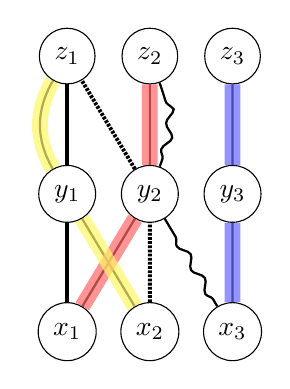
\begin{tikzpicture}[scale=0.7, transform shape = false, rotate=90]
        \pgfkeys{/nodeType/.style={circle, draw},
        /edgeType1/.style={solid, thick, line width=.5mm},
        /edgeType2/.style={solid, thick},
        /edgeType3/.style={thick, decorate, decoration={snake, amplitude=.5mm,pre=lineto,pre length=3pt,post=lineto,post length=3pt}},
        /edgeType4/.style={line width=2mm, draw opacity=0.7}} %highlights the edges of the solution
    
        \def\n{3}
        %n triples (x_i, y_j, z_k) of vertices
        \foreach \i in {1, ..., \n}{
            \node[/nodeType] (x\i) at (0, -1.5*\i) {$x_\i$}; 
            \node[/nodeType] (y\i) at (2.5, -1.5*\i) {$y_\i$}; 
            \node[/nodeType] (z\i) at (5, -1.5*\i) {$z_\i$};
        }
    
        %Edges
        \draw[/edgeType1] (x1) -- (y1) -- (z1);
        \draw[/edgeType2] (x1) -- (y2) -- (z2);
        \draw[/edgeType2] (x2) -- (y1) to[bend left=30] (z1);
        \draw[/edgeType1] [dotted, dash pattern=on 1pt off .5pt] (x2) -- (y2) -- (z1);
        \draw[/edgeType3] (x3) -- (y2);
        \draw[/edgeType3] (y2) to[bend right=20](z2);
        \draw[/edgeType2] (x3) -- (y3) -- (z3);
    
        %Solution
         \draw[/edgeType4] [red!60] (x1) -- (y2) -- (z2);
         \draw[/edgeType4] [yellow!60] (x2) -- (y1) to[bend left=30] (z1);
         \draw[/edgeType4] [blue!60] (x3) -- (y3) -- (z3);    
    \end{tikzpicture}
}
\caption{A \TDMT{} input instance}
\label{fig:sample3dm3}
\end{subfigure}
\quad
\begin{subfigure}[b]{0.58\textwidth}
\centering
\begin{tikzpicture}[scale=0.85, transform shape = false, rotate=90]
    \pgfkeys{/edgeType1/.style={solid, thick, line width=.5mm},
    /edgeType2/.style={solid, thick},
    /edgeType3/.style={thick, decorate, decoration={snake, amplitude=.5mm,pre=lineto,pre length=5pt,post=lineto,post length=5pt}},
    /edgeType4/.style={line width=2mm, green!60, draw opacity=0.7}} %highlights the edges of the solution

    %All vertices
    \node[circle, draw] (x1) at (-1.0, -1.25) {$x_1$};
    \node[circle, draw] (z1) at (4-0.5, -1.25) {$z_1$};
    \setVi{1}{0}{0}{2}
    \node[circle, draw] (x2) at (-1.0, -4.25) {$x_2$};
    \node[circle, draw] (z2) at (4-0.5, -4.25) {$z_2$};
    \setVi{2}{0}{-2.85}{3}
    \node[circle, draw] (x3) at (-1.0, -7.3) {$x_3$};
    \node[circle, draw] (z3) at (4-0.5, -7.3) {$z_3$};
    \setVi{3}{0}{-6.8}{1}

    %Edges
    \draw[/edgeType1] (x1) -- (y111);
    \draw[/edgeType1] (y112) -- (z1);
    \draw[/edgeType2] (y111) -- (y112);
    \draw[/edgeType2] (x2) -- (y121) -- (y122) -- (z1);
    \draw[/edgeType2] (x1) -- (y211) -- (y212) -- (z2);
    \draw[/edgeType1] [dotted, dash pattern=on 1pt off .5pt] (x2) -- (y221);
    \draw[/edgeType2] (y221) -- (y222);
    \draw[/edgeType1] [dotted, dash pattern=on 1pt off .5pt] (y222) -- (z1);
    \draw[/edgeType3] (x3) -- (y231);
    \draw[/edgeType2] (y231) -- (y232);
    \draw[/edgeType3] (y232) -- (z2);
    \draw[/edgeType2] (x3) -- (y311) -- (y312) -- (z3);

    %Solution
    \draw[/edgeType4] [red!60] (x1) -- (y211);
    \draw[/edgeType4] [red!60] (y212) -- (z2);
    \draw[/edgeType4] (y221) -- (y222);
    \draw[/edgeType4] (y231) -- (y232);
    \draw[/edgeType4] [yellow!60] (x2) -- (y121);
    \draw[/edgeType4] [yellow!60] (y122) -- (z1);
    \draw[/edgeType4] (y111) -- (y112);
    \draw[/edgeType4] [blue!60] (x3) -- (y311);
    \draw[/edgeType4] [blue!60] (y312) -- (z3);
\end{tikzpicture}
\caption{The corresponding \GRC{} instance}
\label{fig:sampleGRC}
\end{subfigure}
    \caption{
    A \TDMT{} instance example where $T=\{(x_1, y_1, z_1), (x_1, y_2, z_2),\\ (x_2, y_1, z_1), (x_2, y_2, z_1), (x_3, y_2, z_2), (x_3, y_3, z_3)\}$. Distinct edge types are assigned to each triple, with a solution highlighted.
    The right image depicts the possibility graph of the reduced \GRC{} instance, with a feasible realization highlighted.
    }
    \label{fig:3dm3red}
    \vspace{-.5cm}
\end{figure}

% =>
If a feasible matching $M \subseteq T$ exists in the \TDMT{} instance, we can map it directly to the edges of a valid realization $G$ for the constructed \GRC{} instance.
%
For each $(x_{i_u}, y_j, z_{k_u}) \in M$, using the $u$th occurrence of $y_j$, we add the edges $x_{i_u} y^j_{u,a}$ and $y^j_{u,b} z_{k_u}$ to $G$. For each $(x_{i_v}, y_j, z_{k_v}) \in T \setminus M$, we add the edge $y^j_{v,a} y^j_{v,b}$.
%
Since $M$ is a solution, each vertex in $X \cup Z$ has degree one, satisfying the degree constraints.
%
Additionally, within each group $V_j$, exactly two vertices—$y^j_{u,a}$ and $y^j_{u,b}$ from a triple in $M$—connect to vertices in $X$ and $Z$, respectively. All other vertices within $V_j$ correspond to triples not included in $M$, forming a matching within $V_j$.
%
Therefore, $G$ fulfills both the degree sequence \texttt{d} by assigning degree one to every vertex and the cut list $\mathcal{L}$, meeting all the required constraints for a valid realization.

% <=
Conversely, if a graph $G$ exists that realizes both the degree sequence \texttt{d} and the cut list $\call$, we can construct a feasible matching $M \subseteq T$ for the \TDMT{} instance.
%
Since \texttt{d} specifies a degree of one for each vertex, the edges of $G$ form a matching.
%
Additionally, exactly two vertices within each group $V_j$ are matched to vertices of $X\cup Z$, meaning the remaining vertices within each $V_j$ form an internal matching.
%
These two externally matched vertices must correspond to the same triple in $T$; otherwise, the remaining vertices in $V_j$ could not be paired and meet the type $(V_j, 2)$ cut constraint.
%
Let $M$ consist of the triples in $T$ for which the associated $y^j_{u,a}$ and $y^j_{u,b}$ vertices in $V_j$ are connected to vertices in $X$ and $Z$, respectively.
%
Thus, by construction, vertex $x_i$ connects to $y^j_{u,a}$ and $y^j_{u,b}$ to $z_k$ if and only if the triple $(x_i, y_j, z_k)$ of $T$ belongs to $M$.
%
So $M$ contains exactly one triple per $V_j$, covering each element of $Y$ exactly once, thus $|M| = n$.
%
Since $G$ realizes $\call$, no edges exist between vertices in $X$ and $Z$. Hence, given that $G$ is a matching, each vertex in $X$ connects to exactly one vertex in $Y_a$, and each vertex in $Z$ connects to exactly one vertex in $Y_b$.
%
Consequently, $M$ constitutes a valid matching for the \TDMT{} instance.
\qed
\end{proof}



\section{Final Remarks}
\label{sec:final_remarks}
%resumo do que fizemos
We introduced the \textsc{Graph Realization with Cut Constraints} problem in this work. %, a generalization of the \GRfull{} problem.
%
This problem is interesting because it combines different graph theory concepts, including degree sequence, cut constraints, $f$-factors, and graph realization.
%
We provide a detailed characterization of its computational complexity based on the size of the cuts.
%
Our results show that the problem can be solved in polynomial time when the cuts are small enough (size at most three). However, the complexity significantly increases when the cuts are larger, and we proved that it becomes \classNPH{}.
%
An interesting direction for future work is identifying other graph classes where the possibility graph $\calg$ of a \GRC{} instance ensures polynomial-time solvability. For example, the idea of \cref{prep:tree_graph} might extend to cactus or, more generally, to graphs with bounded degeneracy or treewidth. The case of a planar possibility graph also deserves further investigation. 
%
We also ask about the complexity of {1-in-3 SAT}$_{(2,2)}$, the variant of {1-in-3 SAT} where each variable occurs exactly four times, twice positive and twice negative. 


\begin{credits}
\subsubsection{\ackname}
This work was started during the 6th edition of WoPOCA, which took place in Campinas, São Paulo, Brazil. We thank the organizers and the agencies CNPq (process number 404315/2023-2) and FAEPEX (process number 2422/23).
%
We thank Esther Arkin, Soumya Banerjee, Rezaul Alam Chowdhury, Mayank Goswami, Dominik Kempa, Joseph Mitchell, Valentin Polishchuk, and Steven Skiena for some discussions prior the event, which helped motivate this work.
%
This research has received funding from Rio de Janeiro Research Support Foundation (FAPERJ) under grant agreement E-26/201.344/2021, the National Council for Scientific and Technological Development (CNPq) under grant agreements 309832/2020-9 and \mbox{163645/2021-3}, the São Paulo Research Foundation (FAPESP) under grant agreement 2022/13435-4, and the Brazilian Federal Agency for Support and Evaluation (CAPES) with process numbers 88887.646008/2021-00 and 88887.647870/2021-00. 

\subsubsection{\discintname}
The authors have no competing interests to declare that are
relevant to the content of this article.
\end{credits}

%
% ---- Bibliography ----
%
% BibTeX users should specify bibliography style 'splncs04'.
% References will then be sorted and formatted in the correct style.
%
\bibliographystyle{splncs04}
\bibliography{references}

\end{document}
